\chapter{Lesson Planning}
There are a variety of different types of lesson plan formats that volunteers can use in teaching. The most important thing is that teachers enter the classroom with a lesson plan. Often times, teachers come to class with only their lecture notes, making the lesson unengaging for students, especially those who are not fluent in English. Lessons plans allow us to create interactive lessons that involve the class as a whole and get students interested in the learning material. This develops those qualities of a good learner, as students now want to learn and ask questions. These are the key components to any lesson plan:

\begin{itemize}
\item It must engage or interest the student
\item It should be relevant or be applicable to the students' lives
\item It should encourage the students to think and make their own conclusions
\item It should allow the student to acquire new knowledge
\item It should include lesson notes which are in simple English and written in full sentences
\item It should include the amount of time required for each portion of the lesson and the materials needed
\item It should include a formal or informal assessment of what students have learned
\item It should have notes to improve the lesson in the future
\end{itemize}

\begin{figure}[h!]
\centering
\setlength\fboxsep{0pt}
\setlength\fboxrule{2pt}
\fbox{
\includegraphics[scale=1]{./img/DSC1801.JPG}} 
\end{figure}

In the following pages you will find three types of lesson plans, and an explanation of each.  You can choose one of the following formats or make your own.  Remember, this is your guide for the class and is extremely important to ensure you are teaching engaging and useful lessons for the students, rather than just lecturing at them and hoping they absorb the material.  Further interactive teaching ideas can be found in Chapter 9, Teaching Topics and Ideas.


\newpage

\begin{center}
\section{Engage, Acquire, Practice, Reflect}
\textbf{Developed by PCVs} \\
\end{center}

\begin{flushleft}
First, \textbf{Engage} your students \\
Then, encourage them to \textbf{Acquire} knowledge \\
Third, allow them to \textbf{Practice} what they have learned \\
Final, \textbf{Reflect} together what has been taught and understood \\
\end{flushleft}

\subsection{Activities to Help Students Engage:}
Engage your students in the first 5-10 minutes of class to get them thinking about the topic at hand.
\begin{itemize}
 \item Review Questions
 \item Demonstration
 \item Hands-on experiments
 \item Definition Scramble
 \item Race (who can draw diagram the quickest, answer problem)
 \item Games (list the most prime numbers in 3 minutes)
 \item Puzzles
 \item Motivating questions 
 \item Brainstorming
\end{itemize}

\subsection{Activities to Help Students Acquire Knowledge:}
Teach your students material in a way that is interactive and fun.  
\begin{itemize}
 \item Interactive Lecturing
 \item Group Work
 \item Hands On Experiments
 \item Projects
\end{itemize}

\subsection{Activities to Help Students Practice and Reflect:}
At the end of class, evaluate whether your students have learned the material and understand its importance.
\begin{itemize}
 \item Scavenger Hunts
 \item Review games
 \item Oral Quizzing
 \item Debate
 \item Essays
 \item Homework
 \item Tests and quizzes
 \item ``Today I Learned...''
\end{itemize}

\newpage
\begin{center}
\textbf{Engage, Acquire, Practice, Reflect\\ \textit{Sample Lesson Plan}}\\
\end{center}
\textbf{\textit{ }}\\

\begin{center}
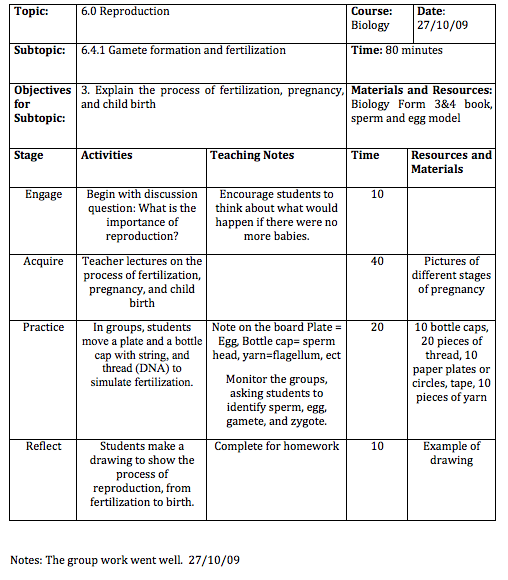
\includegraphics[scale=1]{./img/picture-5.png} 
\end{center}

\newpage
\begin{center}
\section{I Do, You Do, We Do}
\textbf{Developed by Ellen Levy}\\
\end{center}

Scaffolded instruction, sometimes referred to as ``I do it, we do it, you do it'' moves classroom instruction from teacher-centered, whole-group delivery to student-centered collaboration and independent practice.  This method is used in the training of Teach for America Volunteers and was created by Ellen Levy. \\

\begin{center}
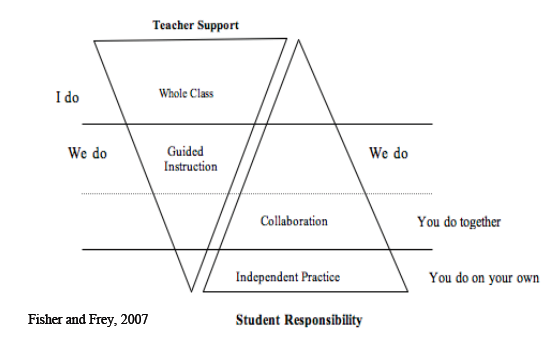
\includegraphics[scale=0.7]{./img/i-do-you-do-triangle.png} 
\end{center}

Taken as a whole, the triangles represent the mentoring relationship and two-way interaction between the teacher and student. At the beginning of a lesson or when new material is being introduced, the teacher has a prominent role in the delivery of the content. This is the ``I do'' phase. But as the student acquires the new information and skills, the responsibility of learning shifts from teacher-directed instruction to student-processing activities. In the ``We do'' phase of learning, the teacher continues to model, question, prompt and cue students; but as students move into the ``You do'' phases, they rely more on themselves and less on the teacher to complete the learning task.

\begin{center}
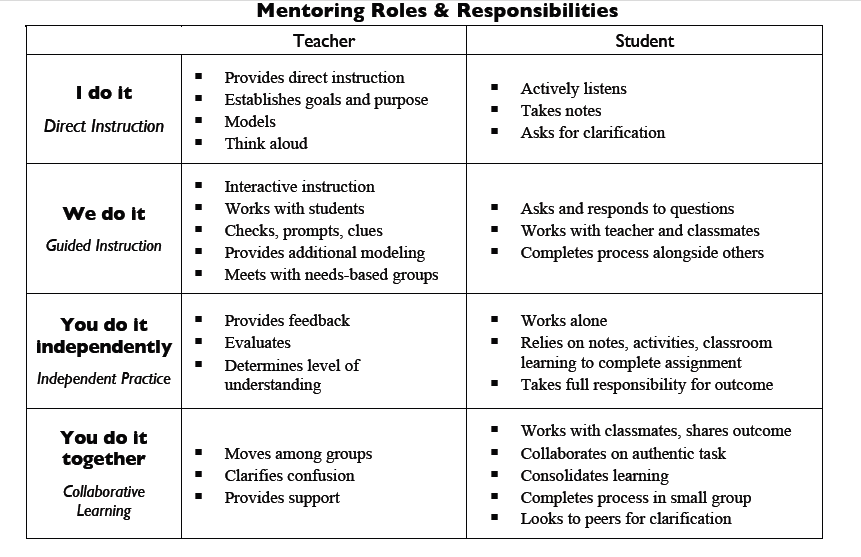
\includegraphics[scale=0.7]{./img/i-do-you-do.png} 
\end{center}

\newpage
\begin{center}
\textbf{I do, We do, You do }\\
\textit{Sample Lesson Plan}
\end{center}

\begin{center}
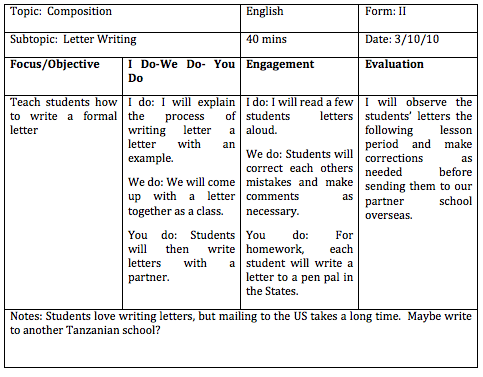
\includegraphics[scale=1]{./img/picture-6.png} 
\end{center}

\newpage
\begin{center}
\section{4MAT}
\textbf{Developed by Bernice McCarthy}\\
\end{center}


4MAT uses the basis of learning profiles and brain modality to develop a 12-step process within a 4-quadrant cycle for learning a given unit or lesson.  This strategy allows you to actively seek to engage every learner through a variety of tactics designed to constantly apply and direct their learning to real-world applications.


\begin{center}
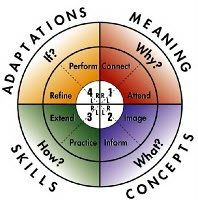
\includegraphics[scale=1]{./img/mat-wheel.jpg} 
\end{center}

\begin{flushleft}
\textbf{Why?} (Quadrant 1 on the wheel)
Answering this question establishes relationships with the content, and personal, meaningful connections based on previous experience.\\

\textbf{What?} (Quadrant 2 on the wheel)
Answering this question allows the student to connect, comprehend, organize, classify and clarify the knowledge.\\

\textbf{How?} (Quadrant 3 on the wheel)
Answering this question allows the student to practice, experiment and get hands-on with the information being presented.\\

\textbf{What If?} (Quadrant 4 on the wheel)
This is where the students will modify, refocus, summarize and ultimately perform the knowledge they have acquired in a real-world context that aids in answering the essential question for the unit or lesson.\\

\end{flushleft}

\newpage
\begin{center}
\textbf{4MAT }\\
\textit{Sample Lesson Plan}
\end{center}

\begin{center}
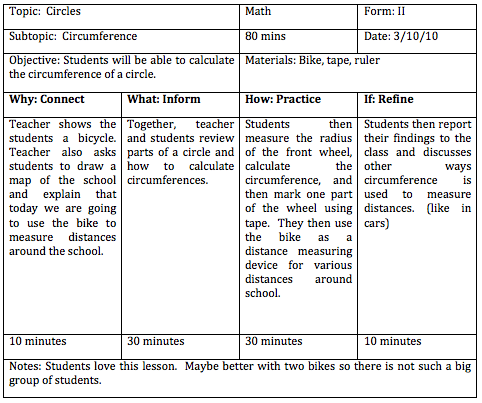
\includegraphics[scale=1]{./img/picture-7.png} 
\end{center}